%! suppress = EscapeHashOutsideCommand
%! suppress = Quote
%! suppress = MissingImport
%! suppress = MissingLabel
%! suppress = LineBreak

% CLI args https://tex.stackexchange.com/a/1501
\newif\ifhandout
\input{flags}

%! suppress = MissingLabel
%! suppress = DocumentclassNotInRoot
%! suppress = DiscouragedUseOfDef

% * Make friends tikz & colors
%   https://en.wikibooks.org/wiki/LaTeX/Colors
% * To enable vertical top alignment globally
%   https://tex.stackexchange.com/questions/9889/positioning-content-at-the-top-of-a-beamer-slide-by-default
% * Set handout from CLI
%   https://tex.stackexchange.com/a/1501
\ifhandout
\documentclass[usenames, dvipsnames, handout]{beamer} % https://tex.stackexchange.com/questions/224091/beamer-how-to-disable-pause-temporarily
\else
\documentclass[usenames, dvipsnames]{beamer}
\fi
% ------------------------------------------------

% Graphics
\usepackage{color}
\usepackage{tabularx}
\usepackage{tikz}
% https://tikz.dev/tikz-graphs
\usetikzlibrary{positioning, shapes.geometric, arrows, automata, graphs}
\tikzset{
    expr/.style={ellipse, draw=gray!60, fill=gray!5, very thick, minimum size=7mm, yshift=0.7cm},
    hexpr/.style={ellipse, draw=gray!60, fill=blue!15, very thick, minimum size=7mm, yshift=0.7cm},
    stmt/.style={rectangle, draw=gray!60, fill=gray!5, very thick, minimum size=5mm, yshift=0.7cm},
    decl/.style={rectangle, draw=blue!60, fill=gray!5, very thick, minimum size=5mm, yshift=0.7cm},
    hdecl/.style={rectangle, draw=blue!60, fill=blue!15, very thick, minimum size=5mm, yshift=0.7cm},
    subtree/.style={shape border rotate=90, isosceles triangle, draw=gray!60, fill=gray!5, very thick, minimum size=5mm, yshift=0.0cm},
}
\usepackage{blkarray}
\usepackage{graphicx}
\usepackage{forest} % https://tex.stackexchange.com/questions/198405/how-to-change-the-color-of-subtrees-in-tikz-qtree
% ------------------------------------------------

% Math
\usepackage{amsmath, amsfonts}
\usepackage{amssymb}
\usepackage{proof}
\usepackage{mathrsfs}
% Crossed-out symbols
% https://tex.stackexchange.com/questions/75525/how-to-write-crossed-out-math-in-latex
\usepackage[makeroom]{cancel}
\usepackage{mathtools}
% ------------------------------------------------

% Additional font sizes
% https://www.overleaf.com/learn/latex/Questions/How_do_I_adjust_the_font_size%3F
\usepackage{moresize}
% Additional colors
% https://www.overleaf.com/learn/latex/Using_colours_in_LaTeX
\usepackage{xcolor}
% Textual math symbols
\usepackage{textcomp}
% ------------------------------------------------

% Language
\usepackage[utf8] {inputenc}
\usepackage[T2A] {fontenc}
\usepackage[english, russian] {babel}
\usepackage{indentfirst, verbatim}
\usetikzlibrary{cd, babel}
% ------------------------------------------------

% Fonts: https://sites.math.washington.edu/~reu/docs/latex_symbols.pdf
\usepackage{stmaryrd}
\usepackage{cmbright}
\usepackage{wasysym}
\usepackage[weather]{ifsym} % https://tex.stackexchange.com/questions/100424/how-to-use-the-ifsym-package
% https://tex.stackexchange.com/questions/615300/pdflatex-builtin-glyph-names-is-empty
\pdfmapline{=dictsym DictSym <dictsym.pfb}
\pdfmapline{=pigpen <pigpen.pfa}
\usepackage{dictsym}
% ------------------------------------------------

% Code
% * Needs -shell-escape build flag
%   https://tex.stackexchange.com/questions/99475/how-to-invoke-latex-with-the-shell-escape-flag-in-texstudio-former-texmakerx
% * Set build directory
%   https://tex.stackexchange.com/questions/339931/latex-minted-package-using-custom-output-directory-build
\usepackage{minted}
\setminted{xleftmargin=\parindent, autogobble, escapeinside=\#\#}
% ------------------------------------------------

% Template
\usetheme{CambridgeUS}
\usecolortheme{dolphin}
% https://tex.stackexchange.com/questions/231439/beamer-how-to-make-font-larger-for-page-numbers
\setbeamerfont{headline}{size=\scriptsize}
\setbeamerfont{footline}{size=\scriptsize}
% Remove heddline
% https://tex.stackexchange.com/questions/33146/how-could-i-remove-a-header-in-a-beamer-presentation
%\setbeamertemplate{headline}{}
% Slide sizes
% https://tex.stackexchange.com/questions/56768/how-to-set-a-small-default-font-size-with-beamer
%\geometry{paperwidth=140mm,paperheight=105mm} % 4:3
\geometry{paperwidth=168mm,paperheight=105mm} % 16:10
% Remove navigation bar
% https://stackoverflow.com/questions/3210205/how-to-get-rid-of-navigation-bars-in-beamer
\beamertemplatenavigationsymbolsempty
% ------------------------------------------------

% Bullets
% https://9to5science.com/change-bullet-style-formatting-in-beamer
% https://tex.stackexchange.com/questions/185742/i-need-to-change-color-of-beamer-itemize-and-subitem-separately
\setbeamertemplate{itemize item}{\scriptsize\raise1.25pt\hbox{\donotcoloroutermaths$\blacktriangleright$}}
\setbeamertemplate{itemize subitem}{\scriptsize\raise1.5pt\hbox{\donotcoloroutermaths$\blacktriangleright$}}
\setbeamertemplate{itemize subsubitem}{\tiny\raise1.5pt\hbox{\donotcoloroutermaths$\blacktriangleright$}}
\setbeamertemplate{enumerate item}{\insertenumlabel.}
\setbeamertemplate{enumerate subitem}{\insertenumlabel.\insertsubenumlabel}
\setbeamertemplate{enumerate subsubitem}{\insertenumlabel.\insertsubenumlabel.\insertsubsubenumlabel}
% ------------------------------------------------

% Table of contents format
% https://tex.stackexchange.com/questions/642927/format-table-of-contents-in-beamer
\setbeamertemplate{section in toc}{%
        {\color{blue}\inserttocsectionnumber.}
    \inserttocsection\par%
}
\setbeamertemplate{subsection in toc}{%
        {\color{blue}\hspace{1em}\scriptsize\raise1.25pt\hbox{\donotcoloroutermaths$\blacktriangleright$}}
    \inserttocsubsection\par%
}
\setbeamertemplate{subsubsection in toc}{%
        {\color{blue}\hspace{2em}\tiny\raise1.25pt\hbox{\donotcoloroutermaths$\blacktriangleright$}}
    \inserttocsubsubsection\par%
}
% ------------------------------------------------

% Misc
\usepackage{multicol}
\usepackage{hyperref}
\usepackage{soul} % https://tex.stackexchange.com/questions/23711/strikethrough-text
% ------------------------------------------------

% Fix \pause for amsmath package envs (black black magic)
% https://tex.stackexchange.com/questions/16186/equation-numbering-problems-in-amsmath-environments-with-pause/75550#75550
% https://tex.stackexchange.com/questions/6348/problem-with-beamers-pause-in-alignments
%! suppress = Makeatletter
\makeatletter
\let\save@measuring@true\measuring@true
\def\measuring@true{%
    \save@measuring@true
    \def\beamer@sortzero##1{\beamer@ifnextcharospec{\beamer@sortzeroread{##1}}{}}%
    \def\beamer@sortzeroread##1<##2>{}%
    \def\beamer@finalnospec{}%
}
%! suppress = Makeatletter
\makeatother
% ------------------------------------------------

% Sections
\newcommand{\sectionplan}[1]{\section{#1}%
    \begin{frame}[noframenumbering]{Содержание}
        \tableofcontents[currentsection]
    \end{frame}
}
\newcommand{\subsectionplan}[1]{\subsection{#1}%
    \begin{frame}[noframenumbering]{Содержание}
        \tableofcontents[currentsubsection]
    \end{frame}
}
% ------------------------------------------------

% Footnotes
\renewcommand{\thefootnote}{\arabic{footnote}}
\renewcommand{\thempfootnote}{\arabic{mpfootnote}}
% https://tex.stackexchange.com/questions/28465/multiple-footnotes-at-one-point
\usepackage{fnpct}
% ------------------------------------------------

% Links
% Colors also links on slide foot.
%\hypersetup{
%    colorlinks=true,
%    citecolor=blue,
%    linkcolor=blue,
%    urlcolor=blue
%}
% ------------------------------------------------

% Appendix
% Slide numbers
% https://tex.stackexchange.com/questions/70448/dont-count-backup-slides
\usepackage{appendixnumberbeamer}
\newcommand{\backupbegin}{
    \newcounter{framenumbervorappendix}
    \setcounter{framenumbervorappendix}{\value{framenumber}}
}
\newcommand{\backupend}{
    \addtocounter{framenumbervorappendix}{-\value{framenumber}}
    \addtocounter{framenumber}{\value{framenumbervorappendix}}
}
% ------------------------------------------------

% Custom commands
% * Decor
\newcommand{\newtopic}[0]{$+$} % item: new topic on "in previous series"
\newcommand{\then}{$\Rightarrow$} % item: consequences
\newcommand{\pop}[0]{\SunCloud} %item:  general eduation
\newcommand{\popslide}[0]{(\pop)}
\newcommand{\advanced}[0]{$\varhexstar$} % item: advanced science
\newcommand{\advancedslide}[0]{(\advanced)}
\newcommand{\practical}[0]{\dstechnical} % item: practical programming notions
\newcommand{\practicalslide}[0]{(\practical)}
\newcommand{\todo}[0]{todo} % item: question
\newcommand{\answer}[0]{\Lightning} % item: answer to the previous question
\newcommand{\eg}[0]{e.g.} % item: example
\newcommand{\defi}[0]{$\Delta$} % item: definition on smth
\newcommand{\textdefi}[1]{\textbf{#1}}
\newcommand{\positive}{$+$} % item: pros
\newcommand{\negative}{{\color{red} $-$}} % item: cons
\newcommand%! suppress = EscapeHashOutsideCommand
\NB[1][0.3]{N\kern-#1em{B}} % default kern amount: -0.3em
\renewcommand{\emph}[1]{{\color{blue} \textit{#1}}}
\newcommand{\vocab}[1]{\textbf{#1}} % item: important new word
% * Lambda calculi
\newcommand{\comb}[1]{\mathbf{#1}} % defined combinator
\newcommand{\term}[1]{\mathbf{#1}} % predefined lambda-term reference
\newcommand{\termdef}{\coloneqq} % lamda term binding
\newcommand{\step}{\rightsquigarrow} % reduction step
\newcommand{\sstep}{\twoheadrightarrow} % multiple steps reduction
\newcommand{\ap}{~} % lambda-term application
\newcommand{\subst}[3]{\left[#2 \mapsto #3 \right] #1} % substitution
\newcommand{\eqbeta}{=_\beta} % beta equality
\newcommand{\eqeta}{=_\eta} % eta-equality
\newcommand{\eqt}{=} % tree-equality of terms
\newcommand{\tlist}[1]{\term{[}#1\term{]}} % list-term
% * Legacy
%\newcommand{\err}[0]{\textcolor{red}{ошибка}} % compilation error

% ------------------------------------------------

% Speaker notes
% https://tex.stackexchange.com/questions/114219/add-notes-to-latex-beamer
% https://tex.stackexchange.com/questions/35444/split-beamer-notes-across-multiple-notes-pages/35496#35496
%\setbeameroption{show notes on second screen=right} % enable speaker notes
%--------------------------------------

\author[]{Андрей Стоян, Илья Колегов, Дмитрий Халанский}
\institute[MSE ITMO]{MSE ITMO}


\title[7. Свёртки]{Практика 7. Свёртки}
\date{осень 2024}

\begin{document}

    \setcounter{framenumber}{-1}
    \maketitle

    \begin{frame}[fragile]{В предыдущих сериях}
        \begin{itemize}
            \item Структуры данных в лямбда-исчислении, операции с ними
            \item Конструкторы данных и паттерн-матчинг в Haskell
            \item Классы типов различных кайндов
            \item[\newtopic] Классы типов \mintinline{haskell}|Semigroup|, \mintinline{haskell}|Monoid|
            \item[\newtopic] Класс типов \mintinline{haskell}|Foldable|
        \end{itemize}
    \end{frame}

    \begin{frame}[noframenumbering]{Содержание}
        \tableofcontents
    \end{frame}

    \sectionplan{Полугруппы и моноиды}

    \begin{frame}[fragile]{Полугруппы и моноиды}
        \begin{itemize}
            \item[\defi] \vocab{Полугруппа} --- множество с ассоциативной бинарной операцией: \mintinline{haskell}|(x <> y) <> z #$\equiv$# x <> (y <> z)|
            \begin{minted}{haskell}
                class Semigroup a where
                  (<>) :: a -> a -> a
            \end{minted}
            \item[\defi] \vocab{Моноид} --- полугруппа с нейтральным элементом: \mintinline{haskell}|x <> mempty #$\equiv$# mempty <> x #$\equiv$# x|
            \begin{minted}{haskell}
                class Semigroup a => Monoid a where
                  mempty :: a
            \end{minted}
            \item[\todo] Сделайте список полугруппой и моноидом
            \item[\todo] Сделайте статистику результатов тестов полугруппой и моноидом
            \mintinline{haskell}|data Counts = Counts { errors :: Int, total :: Int }|
            \item[\todo] Сделайте эндоморфизм полугруппой и моноидом
            \mintinline{haskell}|data Endo a = Endo { getEndo :: a -> a }|
            \item[\todo] Сделайте произвольную функциональную стрелку полугруппой и моноидом
            \item[\todo] Сделайте \mintinline{haskell}|Maybe| полугруппой и моноидом
        \end{itemize}
    \end{frame}

    \begin{frame}[fragile]{Абстракция: цена и новые возможности}
        \vspace{-0.5em}
        \begin{itemize}
            \item В других языках есть всё те же примеры полугрупп, моноидов и т.д., но они не обобщены (как правило)
            \item[\negative] Мозгу тяжело в абстракции без подготовки и тренировки (и всё равно тяжело)
            \item[\negative] Пользователей (программистов) пугают незнакомые слова
            \item[\positive] Можно писать обобщённый код: \mintinline{haskell}|foldMap :: (Monoid m, Foldable f) => (a -> m) -> f a -> m|
            \item[\positive] Обобщённые алгебраические законы гарантируют корректность рефакторинга:
            \begin{center}
                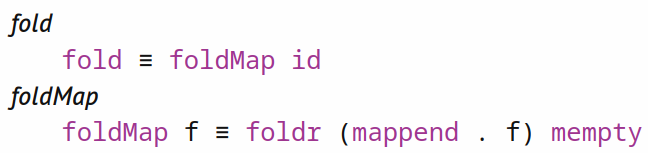
\includegraphics[width=0.5\textwidth]{figs/foldLaws}
            \end{center}
            \item[\positive] Тестирование выполнения реализацией законов можно абстрагировать в библиотеку:
            \begin{minted}{haskell}
                import Test.QuickCheck.Classes.Base
                test = lawsCheck $ foldableLaws $ Proxy @Tree
            \end{minted}
            \item[\positive] Намного проще понять новое, увидев в этом лишь пример знакомой общей концепции
            \item[\positive] Компилятор имеет богатые возможности по генерации инстансов стандартных классов
        \end{itemize}
    \end{frame}

    \sectionplan{Свёртки}

    \begin{frame}[fragile]{Правая свёртка списка или \ldots\footnote{За картинки спасибо Михаилу Беляеву.}}
        \vspace{-1em}
        \begin{columns}[onlytextwidth]
            \begin{column}{0.485\textwidth}
                \begin{minted}{haskell}
                    foldr :: (a -> b -> b) -> b -> [a] -> b
                    foldr f z [] = z
                    foldr f z (x:xs) = f x (foldr f z xs)
                \end{minted}
            \end{column}\hfill%
            \begin{column}{0.5\textwidth}
                \begin{center}
                    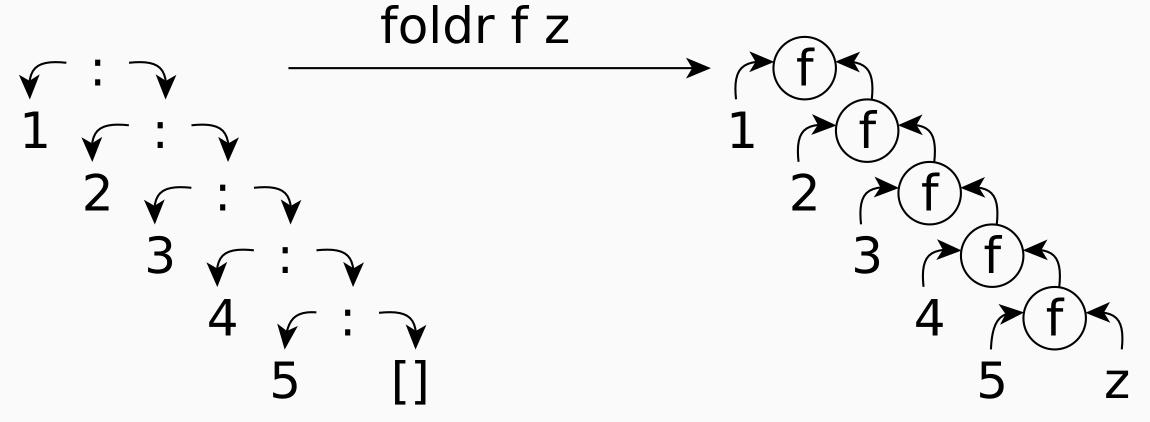
\includegraphics[width=1\textwidth]{figs/foldr}
                \end{center}
            \end{column}
        \end{columns}
        \vspace{0.5em}
        \begin{itemize}
            \item \mintinline{haskell}|foldr f z [a, b, c] #$\equiv$# f a (f b (f c z))|
            \item[\then] То есть списки Чёрча --- свёртка списков через \mintinline{haskell}|data|
            \begin{itemize}
                \item Аналогично и другие структуры данных чистого лямбда-исчисления
                \item А с такими структурами можно, как мы убедились, делать всё то же самое
            \end{itemize}
        \end{itemize}
    \end{frame}

    \begin{frame}[fragile]{Задачки на правую свёртку списков}
        \vspace{-1em}
        \begin{columns}[onlytextwidth]
            \begin{column}{0.485\textwidth}
                \begin{minted}{haskell}
                    foldr :: (a -> b -> b) -> b -> [a] -> b
                    foldr f z [] = z
                    foldr f z (x:xs) = f x (foldr f z xs)
                \end{minted}
            \end{column}\hfill%
            \begin{column}{0.5\textwidth}
                \begin{center}
                    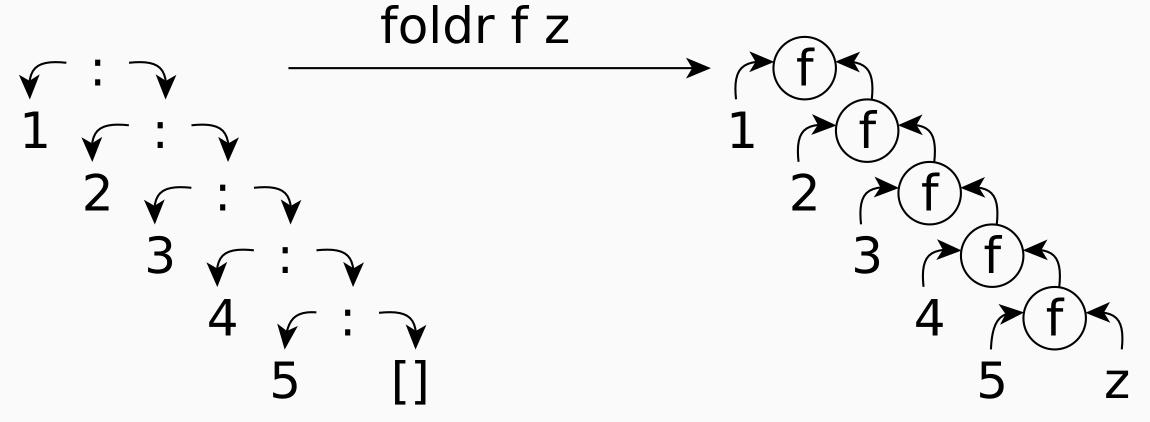
\includegraphics[width=1\textwidth]{figs/foldr}
                \end{center}
            \end{column}
        \end{columns}
        \vspace{0.5em}
        \begin{itemize}
            \item[\todo] Реализуйте скалярное умножение двух векторов, заданных списками
            \item[\todo] Реализуйте группировку пользователей по уровню подписки (\mintinline{haskell}|Data.Map.insertWith :: (a -> a -> a) -> k -> a -> Mak k a -> Map k a|)
            \item[\answer] \pause
             \begin{minted}{haskell}
                 prod xs ys = foldr (*) 1 $ zipWith (+) xs ys
             \end{minted}
            \item[\answer] \pause
            \begin{minted}{haskell}
                group = foldr (\user -> Map.insertWith (++) [subscr user] user) Map.empty
            \end{minted}
        \end{itemize}
    \end{frame}

    \begin{frame}[fragile]{Левая свёртка списков}
        \vspace{-1em}
        \begin{columns}[onlytextwidth]
            \begin{column}{0.485\textwidth}
                \begin{minted}{haskell}
                    foldl :: (b -> a -> b) -> b -> [a] -> b
                    foldl f z [] = z
                    foldl f z (x:xs) = foldl f (f z x) xs
                \end{minted}
            \end{column}\hfill%
            \begin{column}{0.5\textwidth}
                \begin{center}
                    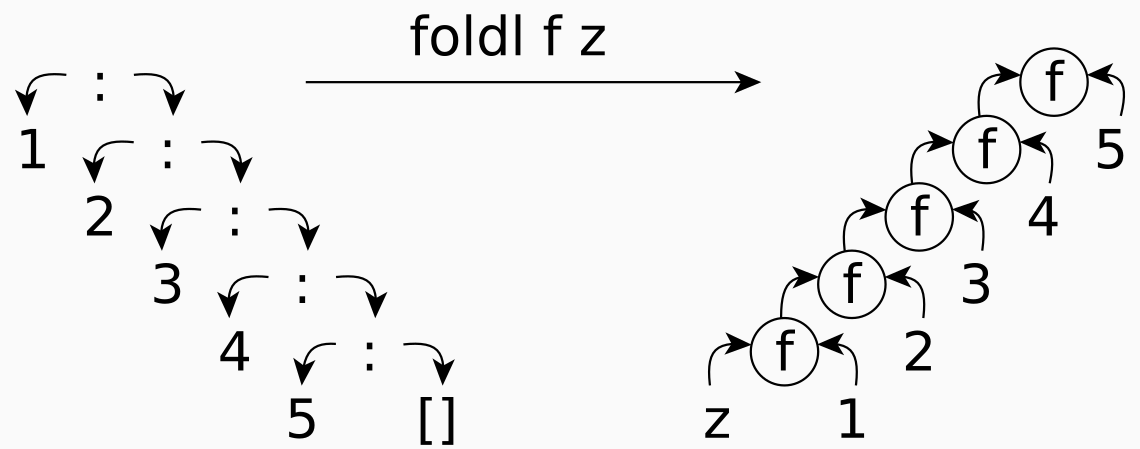
\includegraphics[width=1\textwidth]{figs/foldl}
                \end{center}
            \end{column}
        \end{columns}
        \vspace{0.5em}
        \begin{itemize}
            \item[\todo] Вычтите из чистой прибыли все убытки
            \item[\answer] \pause
            \begin{minted}{haskell}
                income :: Num a => a -> [a] -> a
                income earned expenses = foldl (-) earned expenses
            \end{minted}
        \end{itemize}
    \end{frame}

    \begin{frame}[fragile]{Класс типов \mintinline{haskell}|Foldable|}
        \begin{block}{}
            Коллекции, которые можно обойти и аккумулировать все элементы.
            \begin{minted}{haskell}
                class Foldable (f :: Type -> Type) where
                  foldr :: (a -> b -> b) -> b -> f a -> b
                  foldMap :: Monoid m => (a -> m) -> f a -> m
                  ...
            \end{minted}
        \end{block}
        \begin{itemize}
            \item[\todo] Сделайте пару представителем \mintinline{haskell}|Foldable|
            \item[\todo] Реализуйте \mintinline{haskell}|foldr| через \mintinline{haskell}|foldMap|, что изменится для \mintinline{haskell}|foldl|
            \item[\answer] \pause
            \begin{minted}{haskell}
                instance Foldable ((,) e) where
                  foldMap :: Monoid m => (a -> m) -> (e, a) -> m
                  foldMap f (_, x) = f x
            \end{minted}
            \item[\answer] \pause
            \begin{minted}{haskell}
                foldr f ini xs = foldMap (Endo . f) xs `appEndo` ini
            \end{minted}
        \end{itemize}
    \end{frame}

    \begin{frame}[fragile]{Рецепт приготовления специализированных свёрток}
        \begin{itemize}
            \item Для каждой \mintinline{haskell}|data| существует специализированная свёртка
            \item Заменяем все конструкторы в дереве на функции соответствующих типов
        \end{itemize}
        \begin{enumerate}
            \item Берём функций по числу конструкторов
            \item Типы аргументов --- типы аргументов конструкторов
            \item Рекурсивные типы --- результирующий тип свёртки
        \end{enumerate}
        \begin{minted}{haskell}
            data List a = Nil | Cons a (List a)
            foldList :: List a -> b -> (a -> b -> b) -> b
        \end{minted}
        \begin{itemize}
            \item[\todo]
            \begin{minted}{haskell}
                data Bool = False | True
            \end{minted}
            \item[\todo]
            \begin{minted}{haskell}
                data Nat = Zero | Suc Nat
            \end{minted}
            \item[\todo]
            \begin{minted}{haskell}
                data Nat = Zero | Suc Nat
            \end{minted}
            \item[\answer] \pause
            \begin{minted}{haskell}
                bool :: r -> r -> Bool -> r
                nat :: r -> (r -> r) -> Nat -> r
                uncurry :: (a -> b -> r) -> (a, b) -> r
            \end{minted}
        \end{itemize}
    \end{frame}

    \begin{frame}[fragile]{Работа с коллекциями \practicalslide}
        \begin{block}{Origami Programming}
            <<Recursive equations are the ``assembly language'' of functional programming, and direct recursion the go-to>>
            -- Jeremy Gibbons, Origami Programming (The Fun of Programming), 2003
        \end{block}
        \begin{itemize}
            \item Свёртки наглядно выражают идею аккумулирования коллекции
            \begin{minted}{python}
                state = initial_state
                for x in xs:
                  state = update_state(x, state)
            \end{minted}
            \item Собираем программы из универсальных кирпичиков:
            \begin{minted}{haskell}
                awarded = students  -- (&) :: a -> (a -> b) -> b
                  & map (\(Student name marks) -> (name, average marks))
                  & filter ((> 0) . snd)
                  & foldMap (\(name, s) -> Map.singleton name ("clever cooky: " ++ show s))
            \end{minted}
        \end{itemize}
    \end{frame}

    \sectionplan{Ленивость и выбор свёртки}

    \begin{frame}[fragile]{Ленивая семантика вычислений}
        \vspace{-0.5em}
        \begin{itemize}
            \item В Haskell выражение не вычисляется пока оно не нужно
            \item Что такое нужно? \pause Значение требуется вывести в реальность (e.g.\ напечатать)\footnote{Смешной анекдот: в Haskell любой алгоритм работает за константу (запоминает, что сделать потом).}
            \item Просмотреть, что действительно вычисляется можно в консоли\footnote{Требуется \mintinline{haskell}|:set -XMonomorphismRestriction|. Пользуеся командой \texttt{:sprint}.}
            \begin{columns}[onlytextwidth]
                \begin{column}{0.485\textwidth}
                    \begin{minted}{haskell}
                        take :: Int -> [a] -> [a]
                        take 0 xs = []
                        take n [] = []
                        take n (x:xs) = x : take (n - 1) xs

                        length :: [a] -> Int
                        length [] = 0
                        length (x:xs) = 1 + length xs
                    \end{minted}
                \end{column}\hfill%
                \begin{column}{0.485\textwidth}
                    \begin{minted}{haskell}
                        GHCi> xs = [1, 2 ..]
                        GHCi> :sp xs#\pause#
                        xs = _#\pause#
                        GHCi> ghci> take 1 xs
                        [1]#\pause#
                        GHCi> :sp xs#\pause#
                        xs = 1 : _#\pause#
                        GHCi> ys = [repeat 1, repeat 2]
                        GHCi> length ys
                        2#\pause#
                        ghci> :sp ys#\pause#
                        ys = [_,_]
                    \end{minted}
                \end{column}
            \end{columns}
        \end{itemize}
    \end{frame}

    \begin{frame}[fragile]{Выбор свёртки списка \practicalslide}
        \pause
        \begin{block}{foldr}
            \begin{itemize}
                \item[\positive] \pause Работает с бесконечными списками
                \begin{itemize}
                    \item Правый аргумент \mintinline{haskell}|f| --- результат свёртки на хвосте списка
                    \item Если им не всегда пользоваться, он не будет вычислен
                    \begin{minted}{haskell}
                    and :: [Bool] -> Bool; and = foldr (&&) True
                    -- and [True, False, ...] #$\equiv$# True && (#\framebox{False &&}# #\underline{(... && True)}#)
                    \end{minted}
                \end{itemize}
                \item[\negative] Реализована не через хвостовую рекурсию
            \end{itemize}
        \end{block}
        \begin{block}{foldl}
            \begin{itemize}
                \item[\positive] Реализуется через хвостовую рекурсию --- быстро, может быть компактно
                \begin{itemize}
                    \item Нужно использовать \mintinline{haskell}|Data.List.foldl'| --- энергичную версию
                    \begin{minted}{haskell}
                    foldl' f z (x:xs) = let acc = f z x in acc `seq` foldl' f acc xs
                    \end{minted}
                \end{itemize}
                \item[\negative] Не работает с бесконечными списками
                \begin{itemize}
                    \item Реализация всегда делает рекурсивный вызов на хвосте вне зависимости от \mintinline{haskell}|f|
                \end{itemize}
            \end{itemize}
        \end{block}
    \end{frame}

    \sectionplan{Материалы}

    \begin{frame}{Что посмотреть в транспорте}
        \begin{itemize}
            \item {\color{blue}\url{https://en.wikipedia.org/wiki/Deforestation\_\%28computer\_science\%29}}
            \item \href{https://youtu.be/d3lYx13kdWU?si=ctrQy6pm_44aOgmR}{\color{blue} Лекция Дениса Москвина о функциональном программировании (алгебраические рассуждения и оптимизации работы со списками, fusion)}
        \end{itemize}
    \end{frame}

    \begin{frame}{Материалы}
        \begin{itemize}
            \item \href{https://wiki.haskell.org/GHC\_optimisations\#Fusion}{\color{blue} build/foldr list fusion}
            \item \href{https://www.lektorium.tv/node/32421}{\color{blue} Компилятор GHC языка Haskell: теория языков программирования в работе}
            \item \href{https://hackage.haskell.org/package/stgi}{\color{blue} stgi: Educational implementation of the STG (Spineless Tagless G-machine)}
            \item \href{https://takenobu-hs.github.io/downloads/haskell_ghc_illustrated.pdf}{\color{blue} GHC illustrated}
            \item \href{https://gitlab.haskell.org/ghc/ghc/-/wikis/commentary/compiler/}{\color{blue} GHC Commentary: The Compiler}
            \item \href{https://gitlab.haskell.org/ghc/ghc/-/wikis/commentary/compiler/generated-code}{\color{blue} GHC Commentary: The Compiler: generated code}
        \end{itemize}
    \end{frame}

\end{document}
